\documentclass[a4paper,12pt]{article}

\usepackage[utf8]{inputenc}
\usepackage{graphicx}
\usepackage[dvipsnames]{xcolor}

%\usepackage[defaultmono]{droidmono}
\usepackage{wrapfig}
\usepackage{caption}
\usepackage{subcaption}

\usepackage{amsmath,amssymb,amsthm,textcomp}
\usepackage{ dsfont }
\usepackage{enumerate}
\usepackage{multicol}
\usepackage{tikz}
\usepackage{listings}
%\usepackage{pst-plot}
\usepackage{geometry}
\usepackage{sidecap}
\geometry{total={210mm,297mm},
left=25mm,right=25mm,%
bindingoffset=0mm, top=20mm,bottom=20mm}


\linespread{1.3}

\newcommand{\linia}{\rule{\linewidth}{0.5pt}}

%\savedata{\data}[{{0,0},{1,1},{2,11},{3,6},{4,6},{5,3},{6,2},{7,0},{8,0},{9,1},{10,1},{11,0},{12,1},{13,0},{14,0},{15,0},{16,1},{17,1}}]

%\renewcommand\lstlistingname{Code}

\definecolor{backcolour}{rgb}{0.95,0.95,0.95}

\lstset{%
    backgroundcolor=\color{backcolour},
    basicstyle=\ttfamily\scriptsize,
    breaklines=true,
    captionpos=t,
    numbers=left,
    numberstyle=\tiny,
    numbersep=5pt,
    frame=tb,
    commentstyle=\color{PineGreen},
    keywordstyle=\color{RoyalBlue}
}

% custom theorems if needed
% my own titles
\makeatletter
\renewcommand{\maketitle} {%
\begin{center}
\vspace{2ex}
{\huge \textsc{\@title}}
\vspace{1ex}
\\
\linia\\
\@author \hfill \@date
\vspace{4ex}
\end{center}
}
\makeatother
%%%

% custom footers and headers
\usepackage{fancyhdr}
\pagestyle{fancy}
\lhead{}
\chead{}
\rhead{}
\lfoot{Complex Network \textbar \ Assignment 2}
\cfoot{}
\rfoot{15M54097 - Page \thepage}
\renewcommand{\headrulewidth}{0pt}
\renewcommand{\footrulewidth}{0pt}
%

% code listing settings
%%%----------%%%----------%%%----------%%%----------%%%

\newcommand*{\quoteTitle}[1]{{#1}\ignorespaces}%
\newenvironment{Quote}[1]{
    \medskip\par\noindent\quoteTitle{#1}
    \par\noindent
    \begin{quote}
    }{
    \end{quote}
    \par\noindent\ignorespacesafterend
}

\newtheorem{theorem}{Theorem}

\begin{document}
\bibliographystyle{acm}
\title{Complex Network - Assignment 2}

\author{NGUYEN T. Hoang - SID: 15M54097}

\date{Fall 2015, W833 Mon. Period 5-6 \\ \hfill Due date: 2016/02/01}

\maketitle

\vspace{2em}
\section*{Problem}
\noindent
Given a network as in Figure~\ref{fig:net}. Complete these following tasks:
\begin{enumerate}
    \item Compute eigenvector centrality and betweenness centrality of each vertex in the given network.
    \item Find eigenvectors of matrices, construct the Laplacian and the modularity matrix for this small network:
    \begin{enumerate}
        \item Find the eigenvector of the Laplacian corresponding to the second smallest eigenvalue and hence perform a spectral bisection of the network into two equally sized parts.
        \item Find the eigenvector of the modularity matrix corresponding to the largest eigenvalue and hence divide the network into two communitites.
    \end{enumerate}
    \item Explain quantitatively why ``\emph{your friends have more friends than you do}'' in the configuration model.
    \item Write examples of parameters $\beta$ and $\gamma$ of SIR model when:
    \begin{enumerate}
        \item There is an epidemic.
        \item There is no epidemic.
    \end{enumerate}
\end{enumerate}

\noindent
The source code for this assignment can be found at \cite{mgit}.
\pagebreak
\section*{Answer}

\noindent
In this assignment, I will use SNAP.PY \cite{snap}, a network analysis developed by Stanford University, as a computational tool. All illustrations (figures, graphs \ldots) are drawn using Adobe Illustrator CC 2015.

\paragraph{Question 1:} Compute eigenvector centrality and betweenness centrality of each vertex.

\begin{figure}[h]
    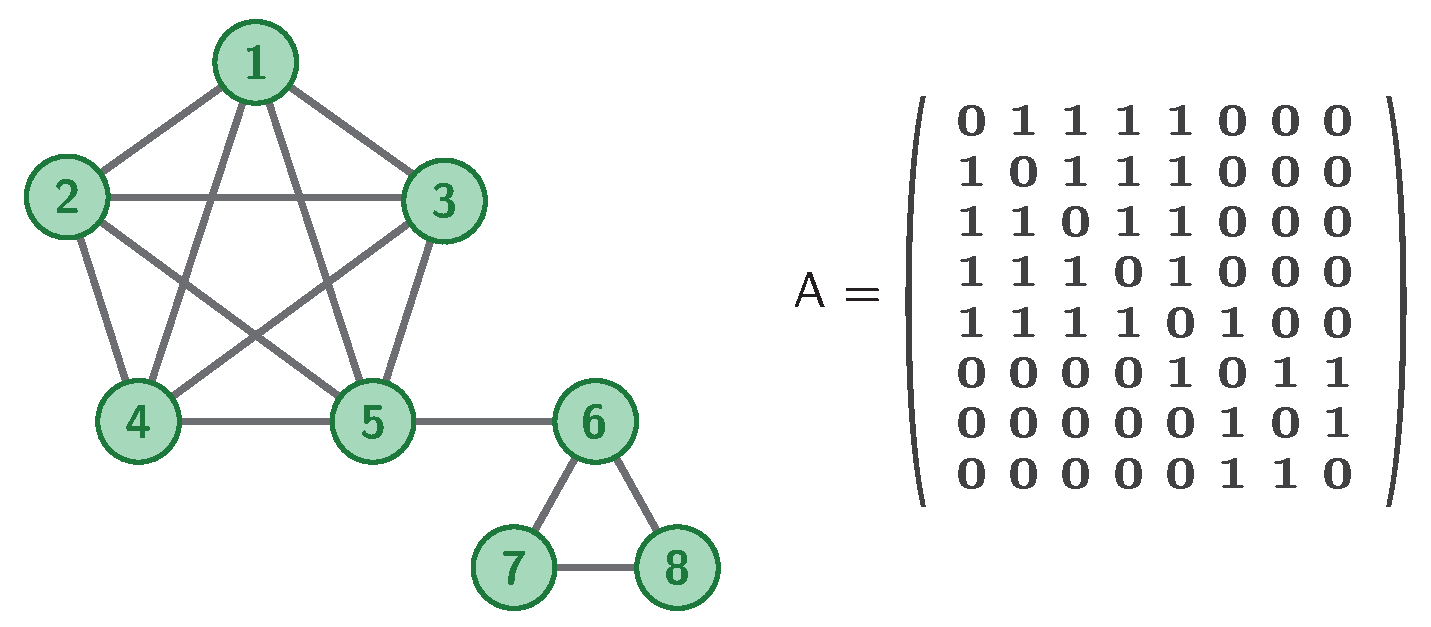
\includegraphics[width=\textwidth]{cn_a2_net}
    \caption{\emph{Simple network and its corresponding adjacency matrix.}}
    \label{fig:net}
\end{figure}

\noindent
\emph{Eigenvector centrality} is given by the formula:
$$ x_i^{(t)}= \underset{j \neq i}{\Sigma} A_{ij} \times x_i^{(t)} $$
Rewrite in final matrix form:
$$ A\boldsymbol{x} = k_1\boldsymbol{x} $$
where $\boldsymbol{x}$ is a vector storing score of all nodes, and $k_1$ is the largest eigenvalue of the adjacency matrix $A$.

\begin{lstlisting}[language=Python, caption={Eigenvector centrality computation with SNAP.PY}, label={lst:eig}]
 # Extracted from UnweightedUndirectedGraph class - File: cn_a2_p1.py
 ...
 import snap as sn
 self._graph = sn.LoadEdgeList(sn.PUNGraph, edge_list, 0, 1, ' ')
 ...
 # Compute eigenvector centrality and store to a hash table.
 def EigenvectorCentrality(self):
     # Create a hash map: Int -> Float
     NIdEigenH = sn.TIntFltH()
     sn.GetEigenVector(self._graph, NIdEigenH)
     return NIdEigenH
\end{lstlisting}

\pagebreak

\noindent
The vector result of Listing~\ref{lst:eig} is shown as follow:
\[ \left( \begin{array}{cccccccc} 0.437 & 0.437 & 0.437 & 0.437 & 0.464 & 0.136 & 0.044 & 0.044 \end{array} \right) \]
\begin{wrapfigure}{r}{0.5\textwidth}
    \vspace{-1em}
    \centering
      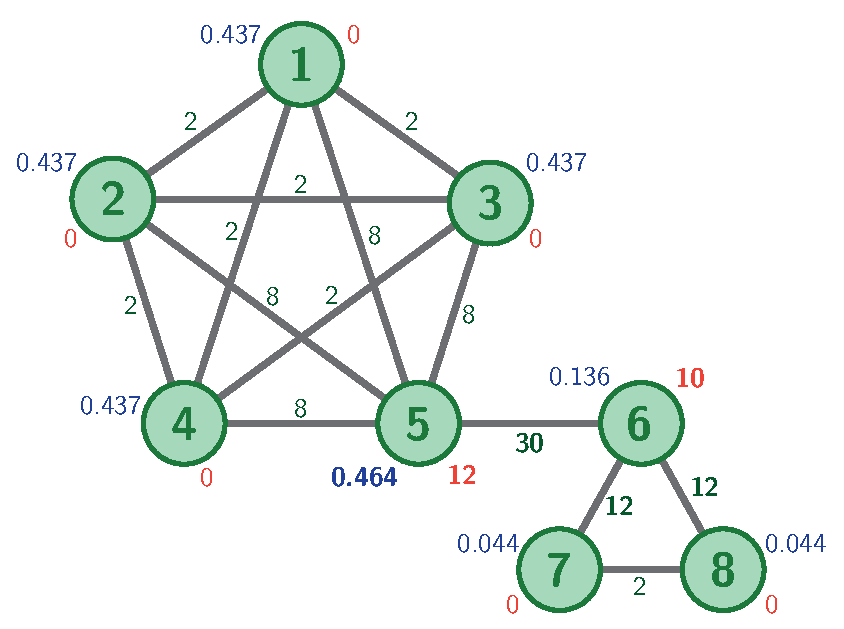
\includegraphics[width=0.48\textwidth]{cn_a2_eigbet}
    \caption{\emph{The given network with eigenvector centrality (blue), and betweenness centrality of vertices (red) and edges (green)}}
    \label{fig:eigbet}
    \vspace{-1em}
\end{wrapfigure}
\noindent
Figure~\ref{fig:eigbet} shows the result in the graph. Eigenvector centrality of each vertex is shown by a blue decimal number next to it. As we can see, vertex number 5 has the highest eigenvector centrality means that vertex number 5 is the most \emph{central} vertex. By looking at the graph, we can intuitively understand this fact.
\newline
\noindent
\emph{Betweenness centrality} is another metric to measure how important a vertex is within the network. Different from other metric, betweenness centrality measure how important a vertex is in the information flow between other vertices. In \cite{net}, the author defines betweenness centrality $x_i$ of vertex $i$ as follow:
$$ x_i = \displaystyle \sum_{st} n_{st}^i \mbox{, or } x_i = \displaystyle \sum_{st} \frac{n_{st}^i}{g_{st}} $$
where $n^i_{st}$ is the number of geodesic paths between vertex $s$ and vertex $t$ that go through $i$, and $g_{st}$ is the total number of geodesic paths between $s$ and $t$. Besides the normal betweenness centrality, in \cite{net} the author also mentioned 2 other types of betweenness: \emph{flow betweenness} and \emph{random walk betweenness}. However, in this assignment, I will only compute the standard betweenness for the given network.

\begin{lstlisting}[language=Python, caption={Betweenness centrality computation with SNAP.PY}, label={lst:bet}]
 # Extracted from UnweightedUndirectedGraph class - File: cn_a2_p1.py
 ...
 import snap as sn
 self._graph = sn.LoadEdgeList(sn.PUNGraph, edge_list, 0, 1, ' ')
 ...
 # Compute betweenness centrality of vertices and edges and store to a hash table.
 def BetweennessCentrality(self, isNode = true):
     # Create 2 hash maps: Int -> Float
     NodeScore = sn.TIntFltH()
     EdgeScore = sn.TIntFltH()
     sn.GetBetweennessCentr(self._graph, NodeScore, EdgeScore, 1.0)
     if (isNode):
         return NodeScore
     else:
         return EdgeScore
\end{lstlisting}

\pagebreak

\noindent
The vector result of Listing~\ref{lst:bet} is shown as follow:
\[ \mbox{NodeScore} = \left( \begin{array}{cccccccc} 0 & 0 & 0 & 0 & 12 & 10 & 0 & 0 \end{array} \right) \]
\[ \mbox{EdgeScore} = \left( \begin{array}{cccccccccccccc} 2 & 2 & 2 & 8 & 2 & 2 & 8 & 2 & 8 & 8 & 30 & 12 & 12 & 2 \end{array} \right) \]
\noindent
Figure~\ref{fig:eigbet} shows the result in the graph. Betweenness centrality of each vertex is shown by a red integer next to it. As we can see, vertex number 5 has the highest betweenness centrality since it is the connection between two cliques.

\paragraph{Question 2:} Construct Laplacian matrix and Modularity matrix for the given network.\\
\noindent
Laplacian matrix and Modularity matrix of the graph is computed with \emph{numpy} as follow:

\begin{lstlisting}[language=Python, caption={Laplacian matrix and Modularity matrix computation with Numpy}, label={lst:mat}]
 # Extracted from UnweightedUndirectedGraph class - File: cn_a2_p1.py
 ...
 import numpy as np
 ...
 self._adj_matrix = edge_list_to_np(edge_list)
 ...
 # Compute and return Laplacian matrix
 def LaplacianMatrix(self):
     D = np.diag(np.sum(self._adj_matrix, 0))
     return D - self._adj_matrix
 ...
 # Compute and return Modularity matrix
 def ModularityMatrix(self):
     B = np.zeros(self._adj_matrix.shape)
     d = np.sum(self._adj_matrix, 0)
     m = sum(d)
     for i in range(B.shape[0]):
         for j in range(B.shape[1]):
             B[i,j] = A[i,j] - (d[i] * d[j]) / float(m)
     return B
\end{lstlisting}

\noindent
The result of Listing~\ref{lst:mat} is:

\[ \mathcal{L} = \left( \begin{array}{cccccccc}
4 & -1 & -1 & -1 & -1 & 0 & 0 & 0 \\
-1 & 4 & -1 & -1 & -1 & 0 & 0 & 0 \\
-1 & -1 & -4 & -1 & -1 & 0 & 0 & 0 \\
-1 & -1 & -1 & -4 & -1 & 0 & 0 & 0 \\
-1 & -1 & -1 & -1 & 5 & -1 & 0 & 0 \\
0 & 0 & 0 & 0 & -1 & 3 & -1 & -1 \\
0 & 0 & 0 & 0 & 0 & -1 & 2 & -1 \\
0 & 0 & 0 & 0 & 0 & -1 & -1 & 2 \end{array} \right) \]
\[ \mathcal{B} = \left( \begin{array}{cccccccc}
-0.571 & 0.428 & 0.428 & 0.428 & 0.281 & -0.443 & -0.429 & -0.289 \\
0.428 & -0.571 &  0.428 &  0.428 &  0.285 & -0.423 & -0.229 & -0.229 \\
0.428 &  0.428 & -0.571 &  0.428 &  0.285 & -0.423 & -0.229 & -0.229 \\
0.428 &  0.428 &  0.428 & -0.571 &  0.285 & -0.423 & -0.229 & -0.229 \\
0.285 &  0.285 &  0.285 &  0.285 & -0.892 & 0.464 & -0.356 & -0.356 \\
0.428 & -0.428 & -0.428 & -0.428 &  0.464 & -0.327 &  0.729 &  0.729 \\
0.285 & -0.285 & -0.285 & -0.285 & -0.357 & 0.785 & -0.144 &  0.856 \\
0.285 & -0.285 & -0.285 & -0.285 & -0.357 & 0.785 &  0.856 & -0.144 \end{array} \right)\]

\subparagraph{(a)} Compute the eigenvalue of the Laplacian Matrix, deduce the second smallest eigenvalue, from there perform a spectral bisection on the graph into 2 equal parts.

\begin{lstlisting}[language=Python, caption={Perform Spectral Bisection on the graph}, label={lst:bisec}]
 # Extracted from UnweightedUndirectedGraph class - File: cn_a2_p1.py
 ...
 import numpy as np
 ...
 self._adj_matrix = edge_list_to_np(edge_list)
 ...
 # Compute spectral bisection
 def SpectralBisection(self):
     L = self.LaplacianMatrix()
     # Get eigenvectors of \L
     u , v = np.linalg.eig(L)
     # Get the second smallest eigenvalue and its eigenvector
     i = np.argsort(u)[1]
     eigv = v[:,i]
     partition = np.ones(eigv.shape[0])
     index_sorted_eigv = np.argsort(eigv)
     for i in range(partition.shape[0] / 2, partition.shape[0]):
         partition[index_sorted_eigv[i]] = -1
     return partition
\end{lstlisting}

\noindent
The vector result for this bisection is demonstrated as follow:
\[ \mbox{partition} = \left( \begin{array}{cccccccc} 1 & 1 & 1 & 1 & -1 & -1 & -1 & -1 \end{array} \right) \]

\begin{wrapfigure}{r}{0.5\textwidth}
    \vspace{-2em}
    \centering
      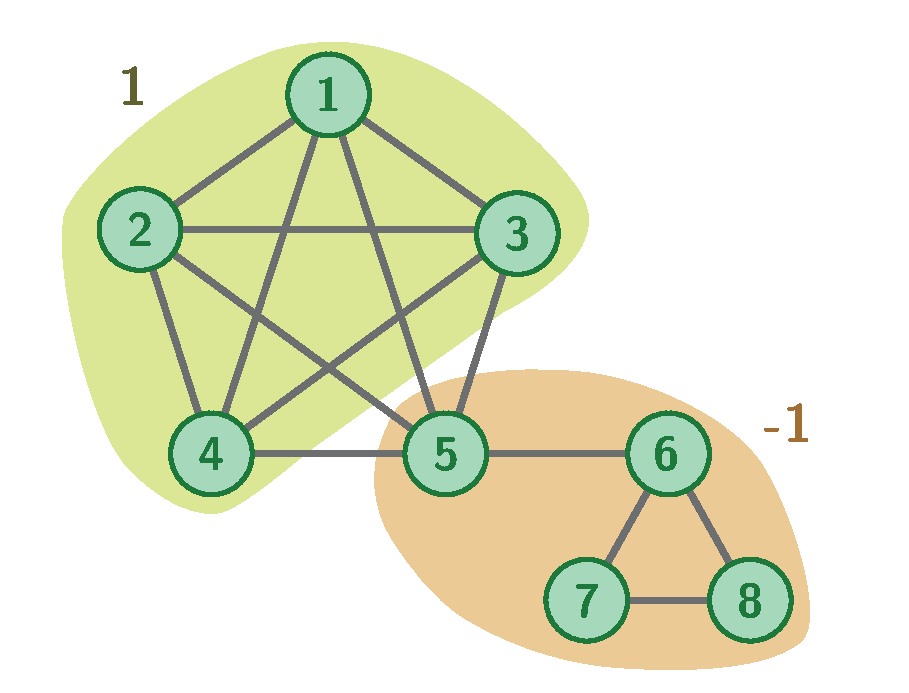
\includegraphics[width=0.48\textwidth]{cn_a2_bisec}
    \vspace{-1em}
    \caption{\emph{Illustration of spectral bisection.}}
    \label{fig:bisec}
    \vspace{-2em}
\end{wrapfigure}

\subparagraph{(b)} Compute the eigenvalue of the Modularity Matrix, deduce the largest eigenvector, from there divide the network into 2 communities.
\noindent
In spectral modularity, we decide groups by possitiveness of each element in the eigenvector. Maximum modularity is archieved when there is a densense connection within a community and sparse between communites. The computation is performed as follow:
\pagebreak

 \begin{lstlisting}[language=Python, caption={Perform Spectral Modularity on the graph}, label={lst:bisec}]
 # Extracted from UnweightedUndirectedGraph class - File: cn_a2_p1.py
 ...
 import numpy as np
 ...
 self._adj_matrix = edge_list_to_np(edge_list)
 ...
 # Compute spectral modularity
 def SpectralBisection(self):
     B = self.LaplacianMatrix()
     # Get eigenvectors of \L
     u , v = np.linalg.eig(L)
     # Get the second smallest eigenvalue and its eigenvector
     i = np.argsort(u)[1]
     eigv = v[:,i]
     partition = np.ones(eigv.shape[0])
     index_sorted_eigv = np.argsort(eigv)
     for i in range(partition.shape[0] / 2, partition.shape[0]):
         partition[index_sorted_eigv[i]] = -1
     return partition
\end{lstlisting}

\noindent
The vector result for this bisection is demonstrated as follow:
\[ \mbox{partition} = \left( \begin{array}{cccccccc} -1 & -1 & -1 & -1 & -1 & 1 & 1 & 1 \end{array} \right) \]

\begin{wrapfigure}{r}{0.5\textwidth}
    \vspace{-2em}
    \centering
      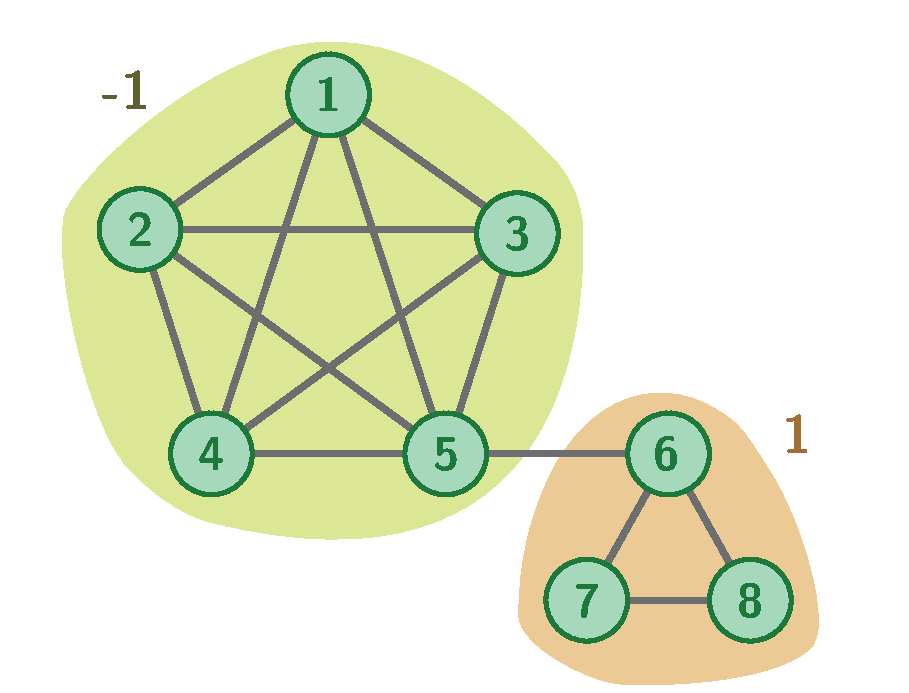
\includegraphics[width=0.48\textwidth]{cn_a2_modul}
    \vspace{-1em}
    \caption{\emph{Illustration of spectral modularity.}}
    \label{fig:modul}
    \vspace{-1em}
\end{wrapfigure}

\noindent
Comparing result between Figure~\ref{fig:bisec} and Figure~\ref{fig:modul}, we can see that the spectral modularity gives us a more \emph{appropriate} result since it divided the given network into two \emph{clique}. Both technique I used here minimizes the number of connection between communities. However, by forcing spectral bisection to divide network into 2 \emph{equal} parts, we obtained an unoptimized result. In conclusion, it is clear that modularity method gives us a better clustering in both computational value and common sense.

\paragraph{Question 3:} Explain quantitatively why ``\emph{your friends have more friends than you do}'' in the configuration model.
\noindent
\emph{Proof: } Suppose we are given a vector $k = \{k_0, k_1, ..., k_{n-1}\}$ contains the degree of all vertices in the configuration model with $n$ vertices and $m$ edges. Without changing the generality of the statement, we assume that $k_i > 0 \forall k_i = \in k$ and $n > 0$. In this context, the word ``friend'' of a vertex $i$ means the adjacency vertices of vertex $i$. Also, $k_i$ is the number of friend that vertex $i$ has. Denote $F_i$ as the number of friends that some vertex $i$ has, and $FF_i$ as the number of friends that friends of vertex $i$ has. Quantitatively, the average number of friend that an arbitary vertex $i$ has is:
$$ \mathds{E}(F_i) = \frac{1}{n} \sum_{i=0}^{n-1} k_i = \frac{2m}{n} $$
Therefore, in this configuration model, the average friend that ``you'' have is $2m/n$. On the other hand, the probability that there is a connection between vertex $i$ and vertex $j$ ($i$ and $j$ are friends) is:
$$ p(i \leftrightarrow j) = \frac{k_ik_j}{2m - 1} \approx \frac{k_ik_j}{2m} $$
The average number of friends that a friend of vertex $i$ has is:
\begin{equation*}
  \begin{aligned}
\mathds{E}(FF_i) & = \frac{1}{k_i} \sum_{j = 0}^{n-1} p(i \leftrightarrow j) \times k_j \\
& = \frac{1}{k_i} \times k_i \sum_{j = 0}^{n-1} \frac{k_j}{2m} \times k_j \\
& = \frac{1}{2m} \sum_{j = 0}^{n-1} k_j^2 \\
  \end{aligned}
\end{equation*}
Consider the different $\mathcal{D}$ between $\mathds{E}(F_i)$ and $\mathds{E}(FF_i)$. Note that $2m = \sum_{j} k_j$:
\begin{equation*}
  \begin{aligned}
    \mathcal{D} & = \mathds{E}(FF_i) - \mathds{E}(F_i) \\
    & = \frac{\displaystyle\sum_{j = 0}^{n-1} k_j^2}{2m} - \frac{k_ik_j}{2m} \\
    & = \frac{n \displaystyle\sum_{j = 0}^{n-1} k_j^2 - 2 \left(\sum_{j = 0}^{n-1} k_j \right)^2 }{2mn} \\
  \end{aligned}
\end{equation*}
Expand the square term $2(...)^2$, we have the following result:
$$\mathcal{D} = \frac{(n-1) \displaystyle\sum_{j = 0}^{n-1} k_j^2 - 2 \sum_{i < j} k_ik_j}{2mn}$$
Using the Cauchy-Schwarz inequality, we have:
$$ k_i^2 + k_j^2 \geq 2k_ik_j $$
Therefore, using the general from of Cauchy-Schwarz we have:
$$ (n-1) \sum_{j = 0}^{n-1} k_j^2 \geq 2 \sum_{i < j} k_ik_j $$
Hence,
$$\mathcal{D} = \frac{(n-1) \displaystyle\sum_{j = 0}^{n-1} k_j^2 - 2 \sum_{i < j} k_ik_j}{2mn} \geq 0$$
In conclusion, the different between average number of a friend's friend and your friend is $\mathcal{D} \geq 0$, therefore the statement ``\emph{(on average) your friends have more friends than you do}'' holds true. QED.

\paragraph{Question 4:} Example of parameter $\beta$ and $\gamma$ of SIR model.
\noindent
In the SIR epidepic model, $\beta$ is the infection rate and $\gamma$ is recover (or death) rate. The model is represented as a system of diffirential equation:
$$ \frac{ds}{dt} = -\beta s x, $$
$$ \frac{dx}{dt} = \beta s x - \gamma x, $$
$$ \frac{dr}{dt} = \gamma x $$
where $s, x, r$ are fraction of population that are \emph{subceptible}, \emph{recovered}, and \emph{infectionous} respectively. Since the solution of these diffirential equation is not analytical, numerical method is applied to analize this SIR model. In real-life application, the parameter $\beta$ and $\gamma$ is determined empirically by trying to fit known data with some trial value of $\beta$ and $\gamma$. The result for each value ($s, x, r$) in this exercise is stored in an array, which is indexed my time step. According to \cite{net}, the epidemic happens when $\beta > \gamma$, which means the disease spreads faster than human recovery. I plotted the time graph for 4 cases:

\begin{figure*}[h!]
  \centering
  \begin{subfigure}[b]{0.45\textwidth}
    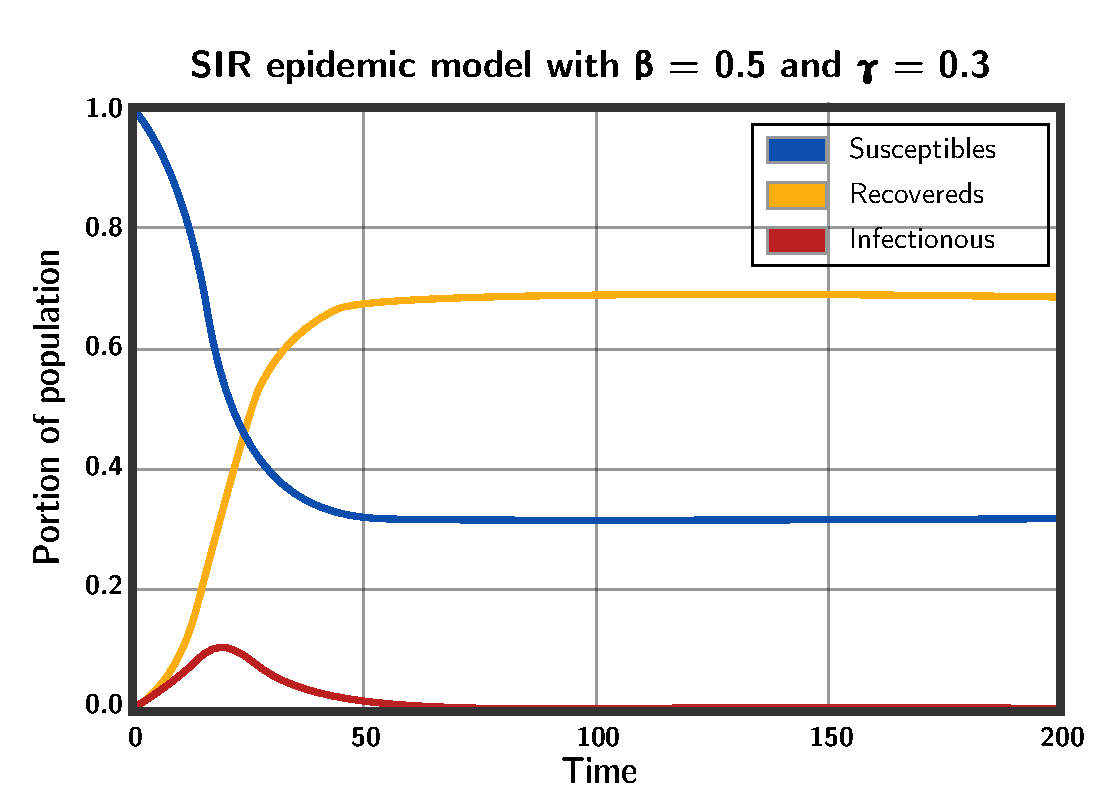
\includegraphics[width=\textwidth]{epidemic1}
    \caption{SIR model, case $\beta = 0.5$ and $\gamma = 0.3$}
  \end{subfigure}
~
\begin{subfigure}[b]{0.45\textwidth}
    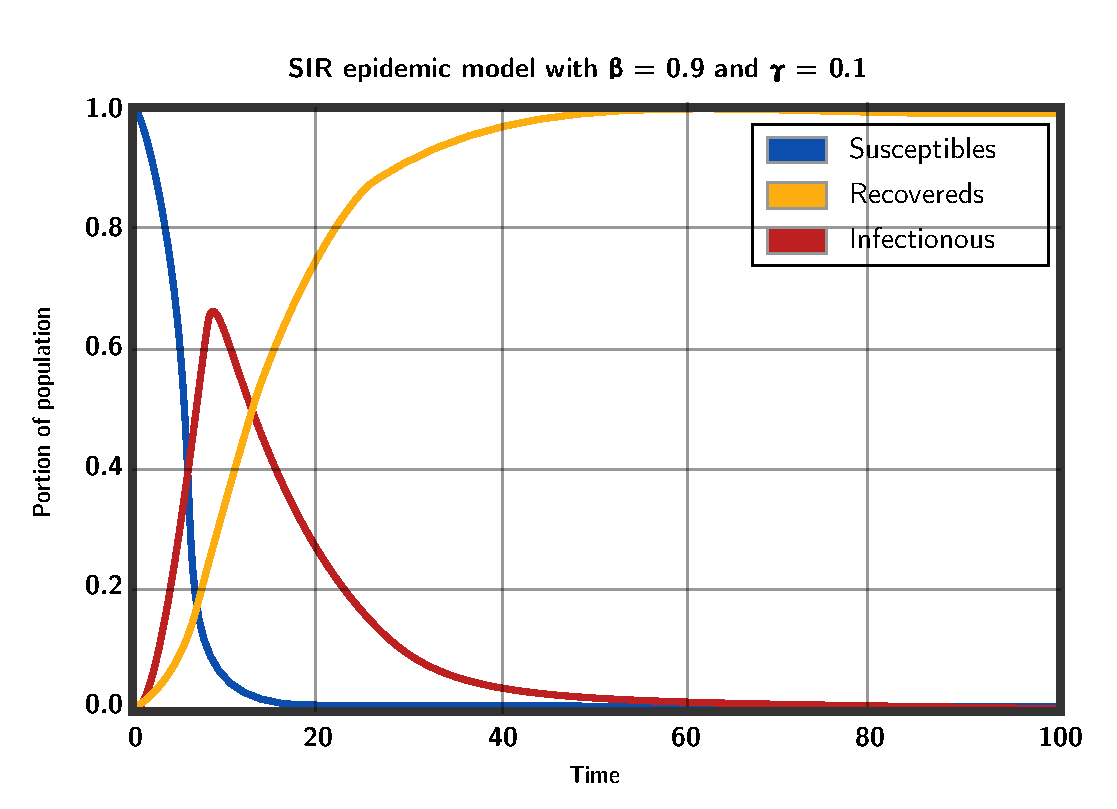
\includegraphics[width=\textwidth]{epidemic2}
    \caption{SIR model, case $\beta = 0.9$ and $\gamma = 0.1$}
  \end{subfigure}
  \caption{SIR model in case of epidemic happens.}
\end{figure*}

\begin{figure*}[h!]
  \centering
  \begin{subfigure}[b]{0.45\textwidth}
    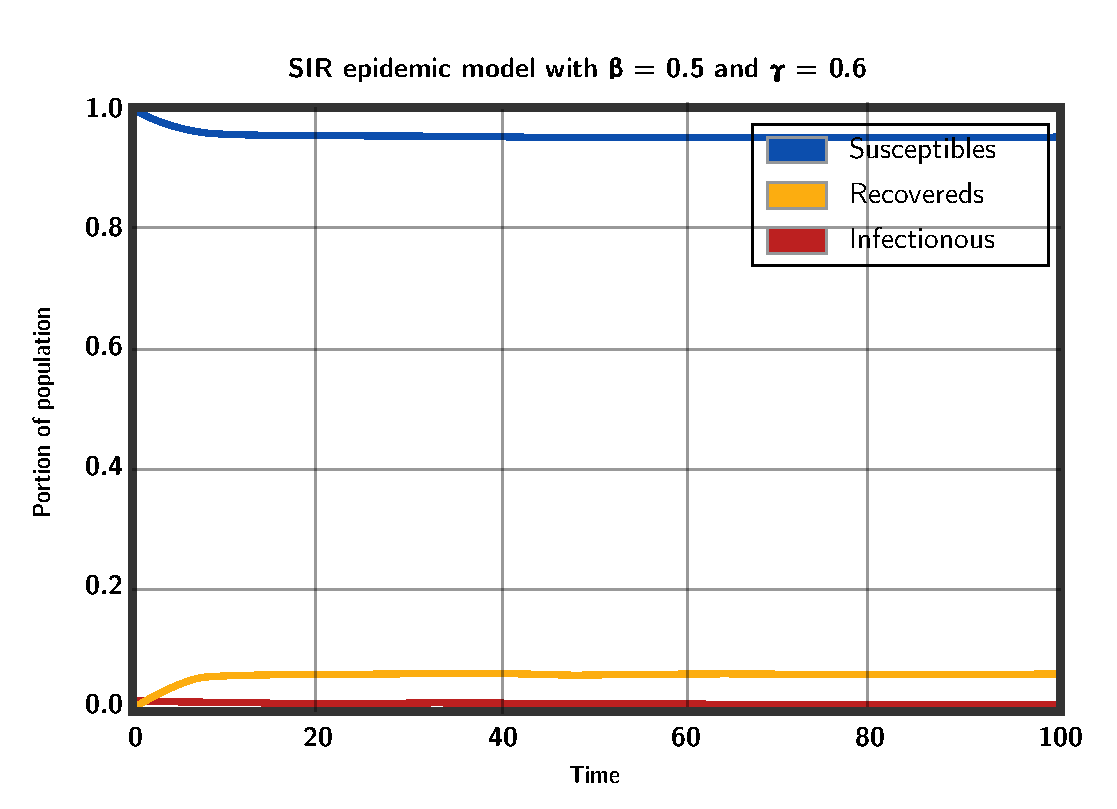
\includegraphics[width=\textwidth]{noepidemic1}
    \caption{SIR model, case $\beta = 0.5$ and $\gamma = 0.6$}
  \end{subfigure}
~
\begin{subfigure}[b]{0.45\textwidth}
    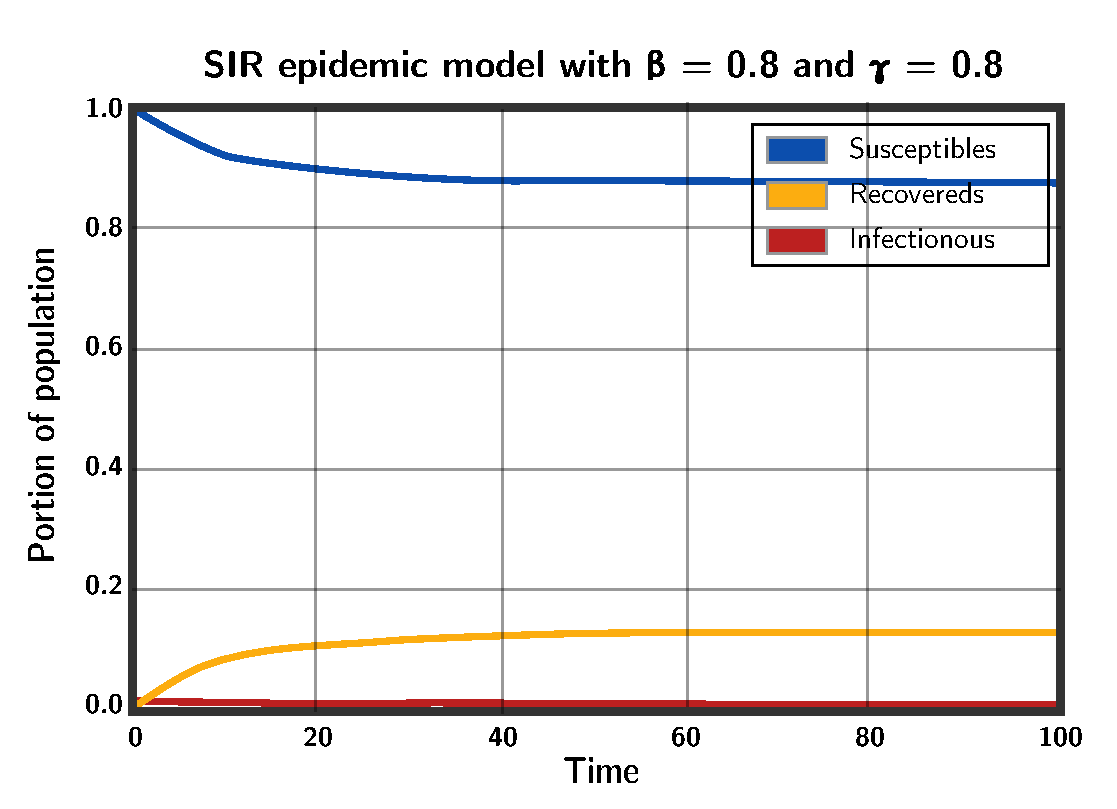
\includegraphics[width=\textwidth]{noepidemic2}
    \caption{SIR model, case $\beta = 0.8$ and $\gamma = 0.8$}
  \end{subfigure}
  \caption{SIR model in case of no epidemic happens.}
\end{figure*}

\bibliography{cn_a2}


\end{document}
